\section{558 --- Quad Tree Intersection}
A quadtree is a tree data in which each internal node has exactly four children: \texttt{topLeft}, \texttt{topRight}, \texttt{bottomLeft} and \texttt{bottomRight}. Quad trees are often used to partition a two-dimensional space by recursively subdividing it into four quadrants or regions.

We want to store \texttt{True}/\texttt{False} information in our quad tree. The quad tree is used to represent a $N \times N$ boolean grid. For each node, it will be subdivided into four children nodes\textbf{ until the values in the region it represents are all the same}. Each node has another two boolean attributes : \texttt{isLeaf} and \texttt{val}. \texttt{isLeaf} is \texttt{true} if and only if the node is a leaf node. The \texttt{val} attribute for a leaf node contains the value of the region it represents.

For example, below are two quad trees $A$ and $B$:


\begin{figure}[H]
\caption{Example $A$}
\centering
\begin{tikzpicture}
%[my/.style={draw, circle, fill=gray!20!, minimum size=5mm}]
\draw[help lines,step=2cm] (0,0) grid (4,4);
\node at (1,1) {$F$};
\node at (3,1) {$F$};
\node at (1,3) {$T$};
\node at (3,3) {$T$};
\end{tikzpicture}
\end{figure}

\begin{figure}[H]
\caption{Example $B$}
\centering
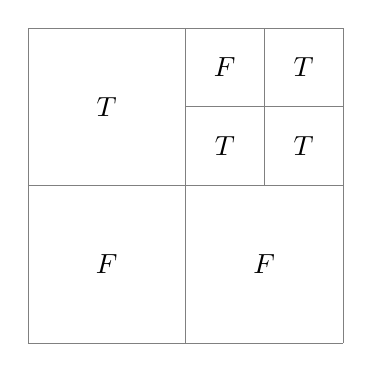
\begin{tikzpicture}
%[my/.style={draw, circle, fill=gray!20!, minimum size=5mm}]
\draw[help lines,step=2cm] (0,0) grid (4,4);
\draw[help lines] (2,2) grid (4,4);
\node at (1,1) {$F$};
\node at (3,1) {$F$};
\node at (1,3) {$T$};
\node at (2.5,2.5) {$T$};
\node at (3.5,2.5) {$T$};
\node at (2.5,3.5) {$F$};
\node at (3.5,3.5) {$T$};
\end{tikzpicture}
\end{figure}

Your task is to implement a function that will take two quadtrees and return a quadtree that represents the logical OR (or union) of the two trees.

\begin{figure}[H]
\begin{minipage}{0.3\linewidth}
\centering
\begin{tikzpicture}
%[my/.style={draw, circle, fill=gray!20!, minimum size=5mm}]
\draw[help lines,step=2cm] (0,0) grid (4,4);
\node at (1,1) {$F$};
\node at (3,1) {$F$};
\node at (1,3) {$T$};
\node at (3,3) {$T$};
\end{tikzpicture}
\end{minipage}
\hfill
\begin{minipage}{0.3\linewidth}
\centering
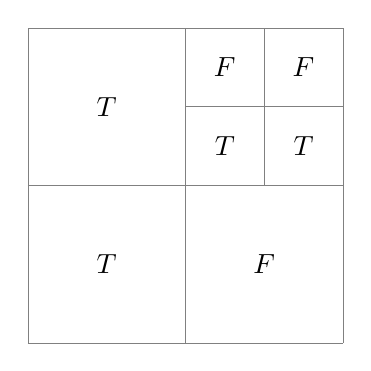
\begin{tikzpicture}
%[my/.style={draw, circle, fill=gray!20!, minimum size=5mm}]
\draw[help lines,step=2cm] (0,0) grid (4,4);
\draw[help lines] (2,2) grid (4,4);
\node at (1,1) {$T$};
\node at (3,1) {$F$};
\node at (1,3) {$T$};
\node at (2.5,2.5) {$T$};
\node at (3.5,2.5) {$T$};
\node at (2.5,3.5) {$F$};
\node at (3.5,3.5) {$F$};
\end{tikzpicture}
\end{minipage}
\hfill
\begin{minipage}{0.3\linewidth}
\centering
\begin{tikzpicture}
\draw[help lines,step=2cm] (0,0) grid (4,4);
\node at (1,1) {$T$};
\node at (3,1) {$F$};
\node at (1,3) {$T$};
\node at (3,3) {$T$};
\end{tikzpicture}
\end{minipage}
\end{figure}

\paragraph{Note:}

\begin{itemize}
\item Both $A$ and $B$ represent grids of size $N \times N$.
\item $N$ is guaranteed to be a power of 2.
\item The logic \textbf{OR} operation is defined as this: $A$ \texttt{or} $B$ is \texttt{true} if $A$ is \texttt{true}, or if $B$ is \texttt{true}, or if both $A$ and $B$ are \texttt{true}.
\end{itemize}

\subsection{Depth First Search}
\begin{itemize}
\item If the one of $A$ and $B$ is leaf and the value is \texttt{True}, the result node is this node. If one of $A$ and $B$ is leaf and the value is \texttt{False}, the result is another node.
\item If both $A$ and $B$ are not leaves, we recursively to get four nodes to represent the intersections of their four child nodes. If these four nodes are all leaves and have same value, we just create and return a new leaf node to store the value.
\item Otherwise, we create and return a non leaf node to store these four nodes.
\end{itemize}

\setcounter{lstlisting}{0}
\begin{lstlisting}[style=customc, caption={DFS}]
Node* intersect( Node* quadTree1, Node* quadTree2 )
{
    if( quadTree1->isLeaf )
    {
        return quadTree1->val ? quadTree1 : quadTree2;
    }

    if( quadTree2->isLeaf )
    {
        return quadTree2->val ? quadTree2 : quadTree1;
    }

    auto tl = intersect( quadTree1->topLeft, quadTree2->topLeft );
    auto tr = intersect( quadTree1->topRight, quadTree2->topRight );
    auto bl = intersect( quadTree1->bottomLeft, quadTree2->bottomLeft );
    auto br = intersect( quadTree1->bottomRight, quadTree2->bottomRight );

    bool one_node = ( tl->isLeaf && tr->isLeaf && bl->isLeaf && br->isLeaf );

    if( one_node )
    {
        if( ( tl->val == tr->val ) && ( bl->val == br->val ) && ( tl->val == bl->val ) )
        {
            one_node = true;
        }
        else
        {
            one_node = false;
        }
    }

    if( one_node )
    {
        auto val = tl->val;
        delete tl;
        delete tr;
        delete bl;
        delete br;
        //create a leaf node represents the four nodes
        return new Node{val, true, nullptr, nullptr, nullptr, nullptr};
    }

    //create a non-leaf node to contains the four nodes
    return new Node{false, false, tl, tr, bl, br};
}
\end{lstlisting}
